\section{Maximale Flüsse in Graphen}

\subsection{Problemstellung}

Sei $G = (V,E,k)$ ein gerichteter Graph mit \begriff{Kapazitätsschranken} $k_e \ge 0$ für alle $e \in E$. Weiterhin sei $q \in V$ einzige \begriff{Quelle} und $s \in V$ einzige \begriff{Senke}. Ohne Einschränkung seien ale Inputdaten ganzzahlig. Für jedes $v \in V$ definieren wir
\begin{equation*}
	E^+(v) \defeq \menge{e \in E : e = (v,p)} \qquad E^-(v) \defeq \menge{e \in E : e = (p,v)}
\end{equation*}
der ausgehenden und eingehenden Bögen für $v$.

\begin{definition}
	Eine Funktion $\abb{x}{E}{\R}$ heißt \begriff{Fluss}, wenn gilt
	\begin{equation*}
		\begin{aligned}
			0 \le x_e \le k_e \quad (e \in E) \\
			\sum_{e \in E^-(v)} x_e = \sum_{e \in E^+(v)} x_e \quad (v \in V \setminus \menge{q,s})
		\end{aligned}
	\end{equation*}
	Die zweite Bedingung (Flusserhaltung) ist auch als \person{Kirchhoff}'sches Gesetz bekannt.
\end{definition}

Die Flusserhaltung impliziert 
\begin{equation*}
	\sum_{e \in E^+(q)} x_e = \sum_{e \in E^-(1)} x_e \defqe f(x)
\end{equation*}
wobei $f(x)$ die Flussstärke angibt.

\begin{beispiel} \label{beispiel: 5.3}
%	(1,2,0/7)
%	(1,3,5/5)
%	(2,3,0/4)
%	(3,5,0/4)
%	(3,4,5/6)
%	(4,2,0/5)
%	(4,5,0/6)
%	(4,6,5/8)
%	(5,6,0/4)

	Dargestellt ist ein zulässiger Fluss der Stärke $f(x) = 5$. Die Bogenmarkierungen entsprechen dabei \enquote{$x_e / k_e$}. Der angegebene Fluss ist nicht optimal.
\end{beispiel}

Ein geeignetes Hilfsmittel zur Prüfung der Optimalität ist der \begriff{Residualgraph} (\enquote{Restgraph}). Ohne Einschränkung nehmen wir an, dass für alle $(u,v) \in E$ auch $(v,u) \in E$ gilt. Sofern dies nicht a priori erfüllt ist, ergänzen wir diese mit Kapazität $k_{(v,u)} = 0$.

\begin{definition}
	Sei $\abb{x}{E}{\R}$ ein zulässiger Fluss, d.h. insbesondere ist $0 \le x_e \le k_e$ für alle $e \in E$. Für $e = (u,v) \in E$ definieren wir
	\begin{equation*}
		r(e) = r(u,v) \defeq k_e - x_e + x_{(v,u)}
	\end{equation*}
	das \begriff{Residuum} (\enquote{Restkapazität}) von $e$.
	Weiterhin sei
	\begin{equation*}
		E(x) \defeq \menge{e \in E : r(e) > 0}
	\end{equation*}
	die Menge aller Bögen mit positiven Residuum\footnote{nur dort besteht die Möglichkeit der Flusserhöhung für den Gesamtgraphen}. Der \begriff{Residualgraph} ist definiert als 
	\begin{equation*}
		G(x) \defeq (V, E(x), r(e)_{e \in E(x)})
	\end{equation*}
	wobei $r(e)$ eine \enquote{aktualisierte Kapazität} beschreibt.
\end{definition}

\begin{beispiel}[Fortsetzung von \labelcref{beispiel: 5.3}]
	Aus dem oben angegebenen Fluss ergibt sich der folgende Residualgraph $G(x)$:
	%	(1,2,/7)
	%	(3,1,/5)
	%	(2,3,/4)
	%	(3,5,/4)
	%	(3,4,/1)
	%   (4,3,/5)
	%	(4,2,/5)
	%	(4,5,/6)
	%	(4,6,/3)
	%   (6,4,/5)
	%	(5,6,/4)
	
	Offenbar gilt stets $r(e) \ge 0$ für alle $e \in E$. $G(x)$ enthält also all jene Bögen, die die Möglichkeit zur Flussvergrößerung modellieren, ergänzt um einige Rückwärtsbögen zur Verminderung von Flüssen auf bisher zu stark genutzten Verbindungen.
\end{beispiel}

Eine mögliche Vorgehensweise zur Erzeugung eines maximalen Flusses ist der folgende Algorithmus:

\fbox{\textbf{Algorithmus von \person{Ford}-\person{Fulkerson}}}
\begin{enumerate}[label=Schritt \arabic*:, leftmargin=*, start=1]
	\item Initialisierung --- Setze $x_e = 0$ für alle $e \in E$ (oder ein \enquote{besserer Startfluss}).
	\item Konstruiere den Residualgraphen $G(x)$. Wenn $G(x)$ keinen Weg von $q$ nach $s$ mit positiver Flussstärke enthält: \texttt{STOP} (Optimalität)
	\item Finde einen Fluss $x'$ in $G(x)$, d.h. einen Weg von $q$ nach $s$ in $G(x)$ mit positiver Flussstärke $f'$. Aktualisiere $x$ gemäßt $x_e \defeq x_e + x_e'$ für alle $e \in E(x)$. Gehe zu Schritt~2.
\end{enumerate}

Bei ganzzahligen Kapazitäten findet in jedem Durchlauf des Algorithmus eine Flussvergrößerung um mindestens eine Einheit statt (sofern er nicht in Schritt~2 abbricht). Damit terminiert das Verfahren nach endliche vielen Schritten. Diese Anzahl an Schritten kann jedoch proportional zum Optimalwert $f^\ast = f(x^\ast)$ sein.
Darüber hinaus gibt es Beispiele mit irrationalen Eingabedaten, für die der obige Algorithmus nicht abbricht.

\subsection{Algorithmus von \person{Edmonds} \& \person{Karp}}

\begin{description}
	\item[Idee:] grundsätzlich analog zu \person{Ford}/\person{Fulkerson}, aber im Schritt~3 wird jeweils ein Weg von $s$ nach $q$ mit kleinster Bogenzahl ermittelt
\end{description}

Es bezeichne $\delta_x(u,v)$ den Abstand zwischen $u \in V$ und $v \in V$ in $G(x)$, also die Anzahl der Bögen auf einem kürzesten Weg von $u$ nach $v$.

\begin{lemma}
	\label{lemma: 5.5}
	Sei $x'$ ein Fluss, der aus dem Fluss $x$ erhalten wird (durch einen flussvergrößernden Weg $P$ in $G(x)$). Dann gilt
	\begin{equation*}
		\delta_x(q,v) \le \delta_{x'}(q,v) \quad \text{ für alle } v \in V \setminus \menge{q}
	\end{equation*}
\end{lemma}
\begin{proof}
	Angenommen es gilt $\delta_x(q,v) > \delta_{x'}(q,v)$ für mindestens ein $v \neq q$. Ohne Einschränkung wählen wir dasjenige $v$ mit minimalem Wert $\delta_{x'}(q,v)$. Also gilt
	\begin{equation}
		\delta_{x'}(q,u) < \delta_{x'}(q,v) \follows \delta_x(q,u) \le \delta_{x'}(q,u)
		\label{eq: 5.1}
	\end{equation}
	weil $v$ das \enquote{minimale Gegenbeispiel} war. Sei $P'$ ein kürzester Weg von $q$ nach $v$ in $G(x')$ und $u$ der letzte Knoten vor $v$. Dann gilt $\delta_{x'}(q,u) = \delta_{x'}(q,v) - 1$ und folglich wegen \eqref{eq: 5.1} 
	\begin{equation}
		\delta_x(q,u) \le \delta_{x'}(q,u)
		\label{eq: 5.2}
	\end{equation}
	Betrachten wir $x(u,v)$ vor der Flussvergrößerung:
	\begin{enumerate}[label=(\alph*), nolistsep]
		\item $x(u,v) < k(u,v)$: Dann ist $(u,v)$ in $G(x)$ vorhanden und es gilt
		\begin{equation*}
			\delta_x(q,v) \le \delta_x(q,u) + 1 \overset{\eqref{eq: 5.2}}{\le} \delta_{x'}(q,u) + 1 = \delta_{x'}(q,v)
		\end{equation*}
		im Widerspruch zur Annahme.
		\item $x(u,v) = k(u,v)$: Dann ist $(u,v)$ nicht in $G(x)$ enthalten, wohl aber $(v,u)$. Da jedoch $P'$ den Bogen $(u,v)$ wieder nutzt, muss dieser in $G(x')$ vorkommen. Das geht nur dann, wenn der flussvergrößernde Weg $P$ (der zum Fluss $x$ gehörte) den Bogen $(v,u)$ enthielt (um somit $x'(u,v) < k(u,v)$ und $(u,v) \in G'(x)$ zu bewirken). Man erhält
		\begin{equation*}
			\delta_x(q,v) \le \delta_x(q,u) - 1 \overset{\eqref{eq: 5.2}}{\le} \delta_{x'}(q,u) < \delta_{x'}(q,v)
		\end{equation*}
		im Widerspruch zur Annahme.
	\end{enumerate}
\end{proof}

Der Algorithmus von \person{Edmonds} und \person{Karp} besitzt eine polynomielle Laufzeit für beliebige (nichtnegative) Kapazitäten.

\begin{lemma}
	Der Algorithmus führt höchstens $\mathcal{O}(\card{V} * \card{E})$ Flussvergrößerungen durch.
\end{lemma}
\begin{proof}
	Jede Flussvergrößerung wird durch einen kritischen Bogen charakterisiert, d.h. auf jedem Weg $P$ gibt es einen Bogen $(u,v)$ mit $r_x(u,v) = \min\menge{r_x(e) : e \in P}$, der die Erhöhung des Flusses am meisten beschränkt. Gemäß Konstruktion verschwindet ein kritischer Bogen im nächsten Schritt aus dem Restgraphen. 
	
	\textbf{Frage:} Wie oft kann ein Bogen $(u,v)$ kritisch werden?  
	Ein kritischer Bogen $(u,v)$ kann in einem späteren Restgraphen wieder auftreten, wenn zuvor $(v,u)$ auf einem flussvergrößernden Weg liegt. Sei $x^0$ ein Fluss, bei dem $(u,v)$ kritisch war. Dann gilt $\delta_{x^0}(q,v) = \delta_{x^0}(q,u) + 1$. Ausgehend von $x^0$ betrachten wir nun die vom Algorithmus erzeugte Folge der Flüsse
	\begin{equation*}
		x^0 \to x^2 \to \dots \to x^t \to \dots \to x^k \qquad (t \neq 0, t \neq k, k \ge 2)
	\end{equation*}
	wobei $(u,v)$ in $x^0$ kritisch ist und das nächste Mal in $x^k$; außerdem wird $(v,u)$ in $x^t$ genutzt. Nun gilt
	\begin{equation*}
		\begin{aligned}
		\delta_{x^k}(q,v) = \delta_{x^k}(q,u) + 1 \overset{\text{\cref{lemma: 5.5}}}{\ge} \delta_{x^t}(q,u) + 1 = \delta_{x^t}(q,v) + 2 \overset{\text{\cref{lemma: 5.5}}}{\ge} \delta_{x^0}(q,v) + 2 
		\end{aligned}
	\end{equation*}
	Also gilt: zwischen zwei Wegen, in denen $(u,v)$ kritisch ist, wächst der Abstand zur Quelle um mindestens zwei Einheiten. Ein solcher Abstand kann höchsten $\mathcal{O}(\card{V})$ Einheiten betragen. Demzufolge kann ein Bogen auch höchstens $\mathcal{O}(\card{V})$ Mal kritisch werden. Insgesamt gibt es höchstens $\mathcal{O}(\card{V} * \card{E})$ Flussvergrößerungen.
\end{proof}

Dies impliziert:
\begin{aussage}
	Der Algorithmus besitzt eine Komplexität von $\mathcal{O}(\card{V} * \card{E}^2)$
\end{aussage}

\begin{beispiel}
%	(1,2,2/5)
%	(1,3,5/5)
%	(2,4,2/6)
%	(3,4,5/5)
%	(3,5,0/4)
%	(4,5,2/2)
%	(5,6,2/4)
%	(4,6,5/5)
Wir betrachten den folgenden Graphen

	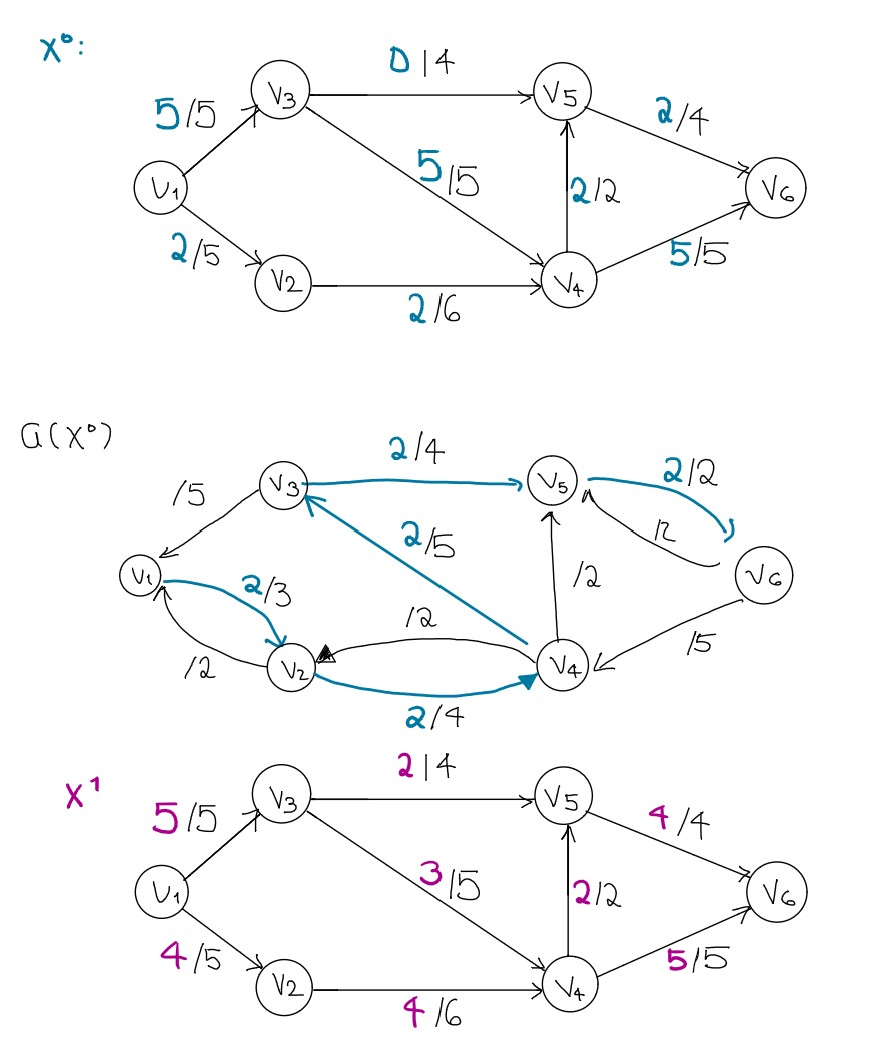
\includegraphics[width=.3\linewidth]{./optinum_abb/optinum_5_4_bsp5-5.jpg}

Flusstärke $= 7$
\end{beispiel}